\begin{frame}
   {Raspberry-pi Zero Serial}
   \begin{figure}[H]
      \centering
      \begin{subfigure}{0.4\textwidth}
         \centering
         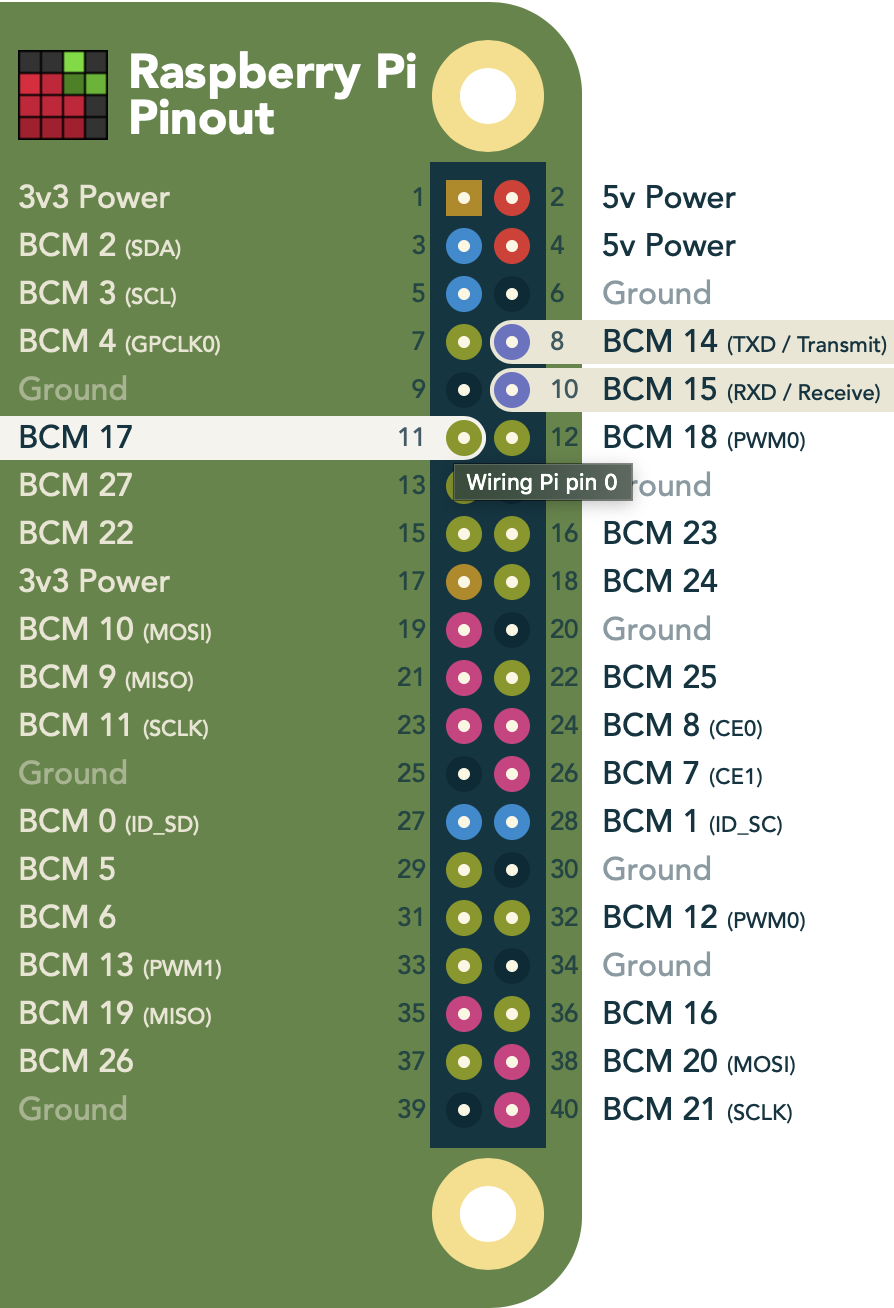
\includegraphics[height=2in]{IMAGES/rpi-pins-uart}
      \end{subfigure}
      \begin{subfigure}{0.4\textwidth}
         \centering
         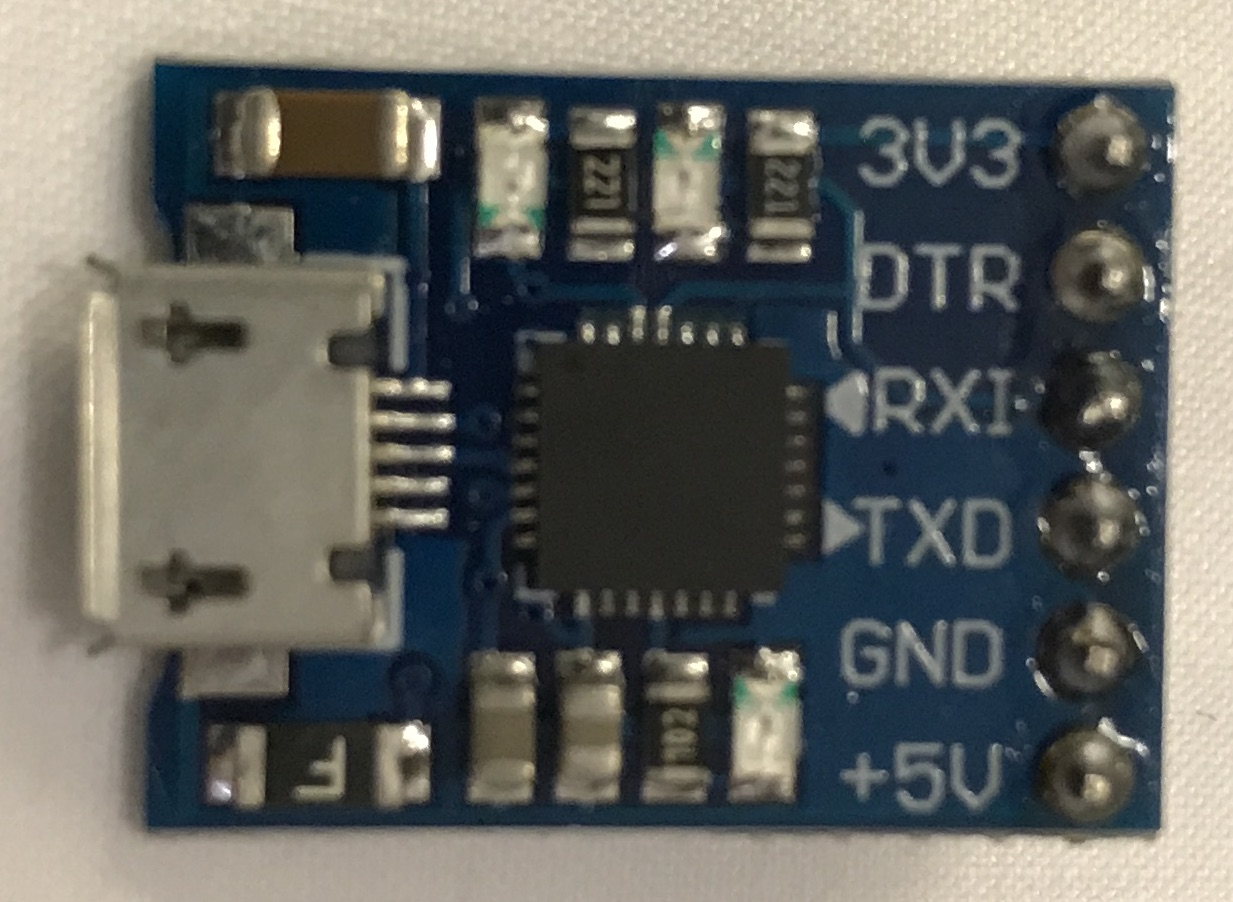
\includegraphics[height=2in]{IMAGES/CP2102}
      \end{subfigure}
   \end{figure}
   \begin{itemize}
      \item We have access to the console serial port through the UART pins using a UART-to-USB converter like the CP2102
      \item We can use this serial port to configure the bootloader and debug kernel issues
   \end{itemize}
\end{frame}

\cprotect\note{

   You can learn more about the \textbf{raspberry-pi serial pins} at pinout.xyz.

   \url{https://pinout.xyz/pinout/uart}
}

